\documentclass[conference]{IEEEtran}
\IEEEoverridecommandlockouts
% The preceding line is only needed to identify funding in the first footnote. If that is unneeded, please comment it out.
\usepackage{cite}
\usepackage{amsmath,amssymb,amsfonts}
\usepackage{algorithmic}
\usepackage{graphicx}
\usepackage{textcomp}
\usepackage{hyperref}
\graphicspath{{images/}}
\def\BibTeX{{\rm B\kern-.05em{\sc i\kern-.025em b}\kern-.08em
    T\kern-.1667em\lower.7ex\hbox{E}\kern-.125emX}}

\newcommand{\Ref}[1]{Fig. \ref{#1}} 
\newcommand{\RefTab}[1]{Table \ref{#1}} 
\begin{document}

\title{Blinking Extraction in Eye gaze System for Stereoscopy Movies}

\author{\IEEEauthorblockN{1\textsuperscript{st} Filip Rynkiewicz}
\IEEEauthorblockA{\textit{Institute of Information Technology} \\
\textit{Lodz University of Technology}\\
Lodz, Poland\\
filip.rynkiewicz@dokt.p.lodz.pl}
\and
\IEEEauthorblockN{2\textsuperscript{nd} Piotr Napieralski}
\IEEEauthorblockA{\textit{Institute of Information Technology} \\
\textit{Lodz University of Technology}\\
Lodz, Poland \\
piotr.napieralski@p.lodz.pl}
}

\maketitle


\begin{IEEEkeywords}
data science algorithms, stereoscopy, blinking extraction, Eye-gaze systems
\end{IEEEkeywords}

\section{Introduction}
Gaze motion research has started in 1879 when French ophthalmologist Louis Emile Javal came to a conclusion that observer does not sweep smoothly along the text with his eyes, but with a series of stops and quick saccades\cite{Winery}.  Since his first observation, the eye-tracking devices were developed. Firstly, those devices were very simple, readers had to wear a type of contact lens with a small opening for the pupil. The lens was attached to a pointer which changed its position following the movements of the eye. The significance of those studies has led to a growth of new, more complicated devices that can automatically measure gaze point. With the rapid advances in information technology, more modern eye tracking devices were developed. These devices give the possibility of detecting a very complex and dynamic factors in the movie environment. These characteristics allow us to evaluate the experience of the viewer \cite{mital2011clustering}.
Using an eye-tracking method to evaluate a viewer's image allows to analyse the experience of the viewer, as well as explore the visual system along with potential processes.
The factors that affect the perception of the image are composed of very complex information. Significant is the provocation of the researched group and its influence on the interpretation of the content conveyed in the film image. Measurement of visual discomfort can be done by monitoring the physiological response of the observer. Such reactions include eye pressure, blink frequency, or electromagnetic activity of the brain \cite{Fornalczyk_Napieralski_Szajerman_Wojciechowski_2015, Fornalczyk_Napieralski_Szajerman_Wojciechowski_20152}.
\section{Human eye anatomy}
Eye is an organ of the visual system, it provides the ability of visual process thus vision. It's origin can be found in photoreceptor proteins that sense light, to simply distinguish between dark and light, found in unicellular organisms. Evolution and adaptation of those simple protein has lead to creation of multiple and very different eye types. Human eye build is not the most complicated in nature, but nevertheless its very sophisticated. For needs of this article the human eye model must by simplified, the diagram can be seen at \Ref{fig:eye_anatomy}
\begin{figure}[!h]
	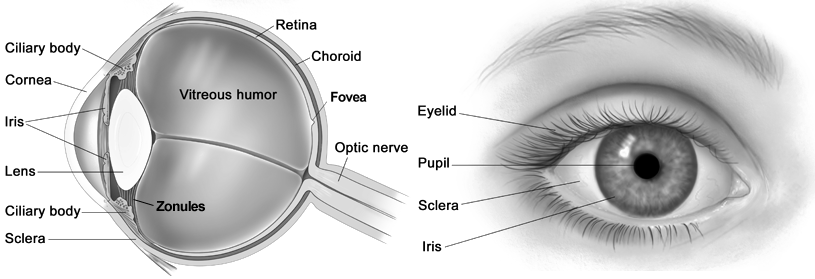
\includegraphics[scale = 0.40]{eye_anatomy.png}
	\caption{Human eye anatomy. Source \url{http://www.relativelyinteresting.com/wp-content/uploads/2011/06/eye+anatomy.png} }
	 \label{fig:eye_anatomy}
\end{figure}
Most important parts of reduced human eye model consist of:
\begin{itemize}
	\item \textbf{Retina} is a light-sensitive layer of tissue.
	\item \textbf{Pupil} is a hole located in the centre of the iris of the eye that allows light to strike the retina.
	\item \textbf{Iris} is a thin, circular structure in the eye, responsible for controlling the diameter and size of the pupil and thus the amount of light reaching the retina.
	\item  \textbf{Eye lid} is a thin fold of skin that covers and protects the human eye
\end{itemize}
\section{Blinking as a factor of visual comfort}
Tracking of eye gaze and movement is based on searching the pupil centre, pupil ellipse, the shape of eye etc. Blinking is most often an involuntary act of shutting and opening the eyelid. When it occurs the eye is automatically closed, so the the position of it will be lost. That's why filtering noise caused by blinking is an important task. The ability to measure the frequency of blinking, allows you to check the observer tiredness. In publications \cite{5606312, 6211573} has been shown that the blink frequency is significantly increased when observing 3D images. Eye fatigue additionally increased blinking frequency. 
\par In conclusion, it can be assumed that the blinking of the eyes varies depending on the conditions: reading, resting or observing 2D or 3D images. The relationship between blinking and visual discomfort of 3D image observation has been investigated, it is resulting from faulty disparity, speed, and type of motion of the scene objects (circular motion on the image plane, static scenes, and inward motion) \cite{00789026}. 
\section{EOG}
One way of extracting the blink is to use the electro-oculogram(EOG). This technique is not new but still there are dozens of research where this technique is used \cite{YagiKunoKogaMukai2006,DenneyDenney1984}. This device is a recording technique that allows the standing potential between the cornea and the posterior pole of the eye to be recorder. Those signals are proportional to the rotational angle of the eye, thus the fixation  point can be detected. Pair of electrodes which are placed at the right and left template and the amplifier are gathering the movement of the eye. Simple scheme can be seen at \Ref{fig:eog}.
\begin{figure}[!h]
	\center
	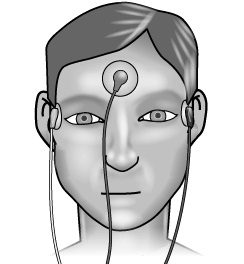
\includegraphics[scale = 0.6]{eog.jpg}
	\caption{Human eye anatomy. Source \url{https://electrooculography.files.wordpress.com/2009/07/eog.gif} }
	\label{fig:eog}
\end{figure}
\begin{figure}[!h]
	\center
	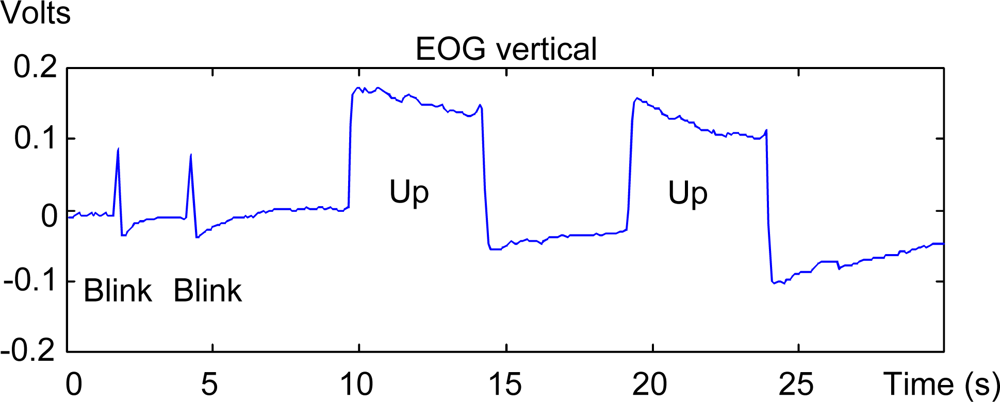
\includegraphics[scale = 0.25]{eog_signal.png}
	\caption{Example of EOG signal. Source \url{http://www.mdpi.com/sensors/sensors-11-00310/article_deploy/html/images/sensors-11-00310f6-1024.png} }
	\label{fig:eog_signal}
\end{figure}
After the signals were collected they need to be processed. Simple EOG signal can be seen at \Ref{fig:eog_signal}. In this example signal of the specific eye movement has been tagged. Tag \textit{UP} is signal equivalent of the eye moving upward, and the \textit{Blink} is blink. In the \textit{Up} the potential is peeking rapidly, remain horizontal for few seconds and then 
dip to original position. The \textit{Down} movement of eye will provide the opposite signal, there will be fast drop then the signal will remain in the same position for few second and in at last will peak to the original position . The \textit{Blink} is the combination of fast \textit{Up} and \textit{Down} movement. So there will be very fast, from 100 to 400 milliseconds(\textit{"Harvard Database of Useful Biological Numbers"}), movement. This can be seen very clearly on the EOG signals.\par The biggest disadvantage of this approach in extracting the blink is that EOG device can affect human emotion. In case where blink might be used to detect visual comfort those little unpleasantness could be significant in research, and give noisier data.
\section{Eye tracker}
Another approach to extracting blink is to use eye tracker device. Those apparatus works on base with infra-red or normal cameras, which track the position of eyes, thus they calculate the gaze of human eye. \par The most common devices are from Tobii and EyeTribe company. The Tobii X2 is a standalone eye-tracker that can be used in various setups by attaching it to the monitors, laptops or for performing eye tracking on physical objects. It has sampling rate 60Hz and system latency under 35ms and it is aimed at determining precisely where the participants are looking, the gaze point, timing, duration of fixations and eye movements such as saccades, for example. This device is using Tobii EyeCore algorithm. 
Second device is also capable of sampling data in 30Hz and 60Hz with less than 20ms latency at 60Hz. This equipment has a way worse precision and has more trouble compensating for users that move their head when being tracked.
\newline\par The output of eye tracker can be seen as the \textit{heat map}, or as \textit{gaze plots}. For this research purpose there was no need to use gaze plots, only the heat map was used \Ref{fig:heat_map}. Those maps show how looking is distributed over the stimulus. There is no information about order of looking in a static heat map.
\begin{figure}[!h]
	\center
	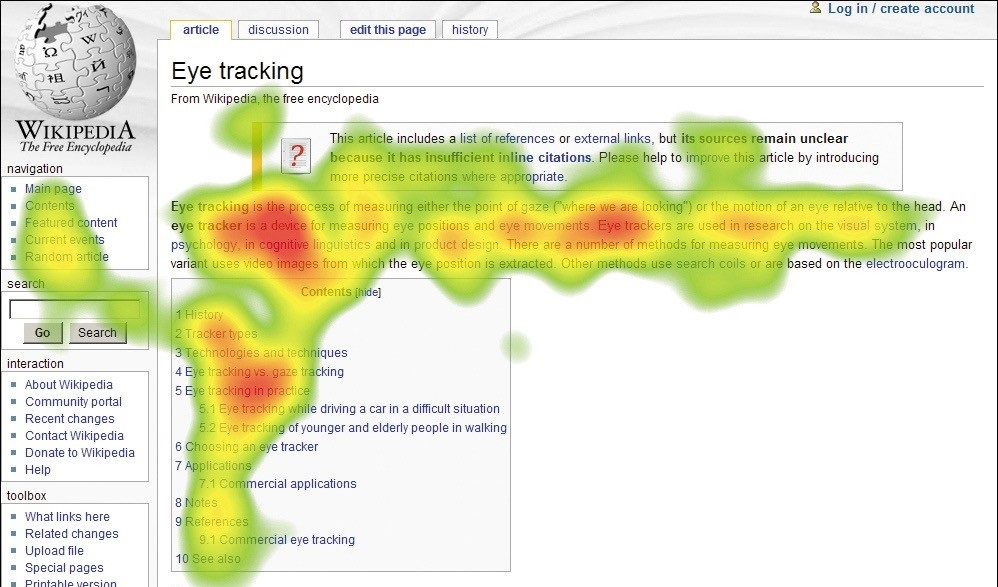
\includegraphics[scale = 0.6]{heat_map.jpg}
	\caption{Example of EOG signal. Source \url{goo.gl/j5N57F} }
	\label{fig:heat_map}
\end{figure}
\section{Methods}
In our research we try to identify reliable blinks, eliminating the noise resulting from measuring blanks. During the research both eye tracker devices, previously described, were tested separately. To increase the reliability of the measurement of the focus points of the viewer's eyes and the correct recording of eye blinks, an additional human face image recorder (GoPro camera) was used to record the face image during the tests. 
\par The 2 people was participated in this research and their task was to watch 5 films each. Every film was from 1:02 to 1:10 minute long, with 10 seconds break between films. In every projection both devices was capturing the eyes, and the face of the examined. Then from data collected by the EyeTracker, blink was extracted and manually compared with the film from camera.
\section{Results}
 Conducted research has shown a relatively complex structure of visual perception, taking into account the experience of the viewer. For the tested devices under the lighting conditions that prevailed at the test site (daylight falling through the window) was unable to register all blinks.
\begin{itemize}
	\item the device often interpreted the squinting as a blink,
	\item the respondents, despite informing them not to move during the study, unfortunately moved on,
	\item other measurement errors \ldots
\end{itemize}
A comparison of the manual analysis of the video recording results and those returned by the EyeTribe indicated that result from the eye-tracker was not as reliable as it was previously thought. The device unexpectedly often interpreted eye loss as a batting factor. The test results became more reliable after replacing the EyeTribe device with Tobii's X2. Blink reliability tests proved to be much better than the EyeTribe, but still not enough.
\par
In \RefTab{tab1} part of our data was showed, and explanation of abbreviations used in it:
\begin{itemize}
	\item \textbf{\textit{time}} $\rightarrow$ time of capturing data in milliseconds,
	\item \textbf{\textit{x}} $\rightarrow$ position of the eyes on 2D plane at x,
	\item \textbf{\textit{y}} $\rightarrow$ position of the eyes on 2D plane at y,
	\item \textbf{\textit{blink$_{et}$}} $\rightarrow$ flag indicates that blink was recognized by EyeTracker,
	\item \textbf{\textit{pd}} $\rightarrow$ pupil diameter,
	\item \textbf{\textit{blink$_{f}$}} $\rightarrow$ flag indicates that blink was recognized on film recorded by GoPro, manually extracted.
\end{itemize}
State when \textbf{\textit{pd}}, \textbf{\textit{x}} or \textbf{\textit{y}} is 0 or -1 indicates that the device detected the eye bink or lost the position of the eye. When the \textbf{\textit{blink$_{et}$}} flag is set to -1 or 0 that indicate that the EyeTracker has recognized blink. 

\begin{table}[htbp]
	\caption{Part of data from experiment 1 with participant 2}
	\begin{center}
		\begin{tabular}{|c|c|c|c|c|c|c|}
			\hline
			 \textbf{\textit{time}}&\textbf{\textit{x}}& \textbf{\textit{y}}& \textbf{\textit{blink$_{et}$}} & \textbf{\textit{pd}} & \textbf{\textit{blink$_{f}$}}  \\ \hline
			 13331 & -1 & -1 & -1 & -1 & 0 \\ \hline
			 13351 & -1 & -1 & -1 & -1 & 0 \\ \hline
			 13392 & 0 & 0 & 0 & 258248 & 0 \\ \hline
			 13419 & 9306 & 582183 & 0 & 257948 & 1 \\ \hline
			 13448 & 0 & 0 & 0 & 250292 & 0 \\ \hline
			 13492 & 0 & 0 & 0 & 249693 & 0 \\ \hline
			 13533 & 281300 & 148322 & 0 & 247866 & 0 \\ \hline
			 55661&	0&	0	&0	&-1&	1 \\ \hline
			\hline
			
			\hline
			\multicolumn{1}{c}{}
		\end{tabular}
		\label{tab1}
	\end{center}
\end{table}
In first column where time was 13331 ms of movie the EyeTracker has detect eye blink, but it was not confirmed on GoPro film.
In next data sample participant has blinked in \textit{13149} ms of movie. That was confirmed on film recorded by GoPro camera, but the EyeTracker does not recognized it. Even in next data sample, 13448ms and 13492ms, where EyeTracker has lost the eye position(\textbf{\textit{x}} \textbf{\textit{y}} are both 0 and \textbf{\textit{pd}} is 250292) this device does not recognized the blink. 
In last column at 55661 the Eyeracker and GoPro camera has both positively identify the eye blink of participant.
\section{Further research}
In our test we found that there is no perfect and reliable solution to extract the blink, because in further research the connection between blink and emotion will be evaluated. The EOG perfectly reveals the  blink, but the diodes and cables can be disturbing to surveyed, thus the emotion recognition could be noised. On the  other hand the eye-tracer device does not always detect the blink, but for user it's less intrusive.  In next researches there is a need to create solution for extracting the blink where the method will be indifferent for the user and could identify blink with the best accuracy possible.

\begin{thebibliography}{00}
\bibitem{Fornalczyk_Napieralski_Szajerman_Wojciechowski_20152}
Fornalczyk, K., Napieralski, P., Szajerman, D., Wojciechowski, A., Sztoch, P.,
Wawrzyniak, J.: Stereoscopic image perception quality factors pp. 129--133
(2015)

\bibitem{Fornalczyk_Napieralski_Szajerman_Wojciechowski_2015}
Fornalczyk, K., Napieralski, P., Szajerman, D., Wojciechowski, A.: Stereoscopic
image visual perception. International Journal of Microelectronics and
Computer Science  6(1),  15--22 (2015)

\bibitem{Winery}
Huey, E.B.: The psychology and pedagogy of reading (1908)

\bibitem{5606312}
Lee, E.C., Heo, H., Park, K.R.: The comparative measurements of eyestrain
caused by 2d and 3d displays. IEEE Transactions on Consumer Electronics
56(3),  1677--1683 (Aug 2010)

\bibitem{00789026}
Li, J., Barkowsky, M., Le~Callet, P.: {VISUAL DISCOMFORT IS NOT ALWAYS
	PROPORTIONAL TO EYE BLINKING RATE: EXPLORING SOME EFFECTS OF PLANAR AND
	IN-DEPTH MOTION ON 3DTV QOE}. In: {International Workshop on Video Processing
	and Quality Metrics for Consumer Electronics VPQM 2013}. pp. pp.1--6.
Scottsdale, United States (Jan 2013)

\bibitem{mital2011clustering}
Mital, P.K., Smith, T.J., Hill, R.L., Henderson, J.M.: Clustering of gaze
during dynamic scene viewing is predicted by motion. Cognitive Computation
3(1),  5--24 (2011)

\bibitem{6211573}
Yu, J.H., Lee, B.H., Kim, D.H.: Eog based eye movement measure of visual
fatigue caused by 2d and 3d displays. In: Proceedings of 2012 IEEE-EMBS
International Conference on Biomedical and Health Informatics. pp. 305--308
(Jan 2012)
\bibitem{YagiKunoKogaMukai2006}
T. Yagi, Y. Kuno, K. Koga and T. Mukai, Drifting and Blinking Compensation in Electro-oculography (EOG) Eye-gaze Interface, 2006 IEEE International Conference on Systems, Man and Cybernetics, Taipei, 2006, pp. 3222-3226.
URL: \url{http://ieeexplore.ieee.org/stamp/stamp.jsp?tp=&arnumber=4274377&isnumber=4274280}
\bibitem{DenneyDenney1984}
Denney D, Denney C. The eye blink electro-oculogram. The British Journal of Ophthalmology. 1984;68(4):225-228.



\end{thebibliography}

\end{document}
